\documentclass[12pt]{article}
\usepackage[margin=1in]{geometry}

%% \usepackage{amsmath}
\usepackage{color}
\usepackage{graphicx}

\usepackage{float} 
\floatstyle{ruled}
%\newfloat{program}{tbp}{lop}[section]
\newfloat{program}{thp}{lop}
\floatname{program}{Program}


%\usepackage{listings}
%% \lstloadlanguages{C++}
%% \lstset{
%%   language=C++, 
%%   breaklines=true,
%%   keywordstyle=\color{blue},
%%   commentstyle=\color{red}
%% }
 

\title{New Multithreaded CPU/GPU Hartree-Fock Implementation}
\author{Andrey Asadchev \and Mark Gordon}
\date{}

\begin{document}

\maketitle 

\abstract{
In this article a new multithreaded Hartree-Fock CPU/GPU
implementation is presented which utilizes automatically generated
code and modern C++ techniques to achieve a significant improvement
with respect to memory and computer time over the legacy fortran code.
}

\section*{Introduction}
As the computer hardware becomes more sophisticated and complex and as the
programming languages, compilers, and software patterns mature, it becomes
necessary to revisit old implementations written in Fortran during the eighties
and even earlier in order to take advantage of modern hardware and software features.

It is evident today, as processors have more and more cores, as multithreading
becomes more and more important, and as novel architectures such as graphical
processor units (GPU) enter mainstream scientific computing, that programs
written years ago do not take advantage of the full power of modern hardware.

On one hand, old programs do not take into account low-level details of modern
processors such as multilayer cache organization, pipelines, and SIMD
units \cite{gerber_software_2006}.
As a result of poor cache performance, programs waste CPU cycles moving memory at
the expense of crunching numbers.  Failure to take advantage of SIMD, which may
be due to unfavorable control structures and memory access patterns, can lead to
as much as 50 percent drop in performance.  The parallel execution within a
single note suffers as well: computational tasks tend to run as processes rather
than threads, limiting the utility of shared memory and fast inter-thread
communication offered by multi-threaded environment
\cite{gerber_programming_2004},
resulting in replicated memory which puts additional strain on memory cache and bus.

This paper describes new implementation of Hartree-Fock method meant
to address the requirements of the modern hardware and software, from low-level
two-electron Rys Quadrature implementation to multi-threaded parallel Fork matrix
construction and GPU implementation.  The paper is organized as follows:

\begin{itemize}
  \item Rys Quadrature Algorithm Ideas
    \begin{itemize}
    \item Automatically generated code
    \item Small shell quartets requirements
    \item Large shell quartets requirements
    \end{itemize}
  \item Fock Matrix Algorithm Ideas
    \begin{itemize}
    \item Block approach to Fock matrix
    \item Collapsing nested loops into a task queue
    \item Multi-threaded implementation
    \item Normalization coefficients
    \end{itemize}
  \item C++ Implementation
  \item GPU Implementation
  \item Performance Results
\end{itemize}


\section*{Rys Quadrature Implementation}
Modern computers have complex architectures and pipelines, making it nearly
impossible for human programmer to write efficient assembly code.  However
modern compilers are able to produce the efficient code if several constraints
are met:

\begin{itemize}
\item Memory access have favorable alignment, 16 bytes for current Intel
  architecture
\item Non-overlapping segments of memory are flagged as such, using special type
  declaration or compiler pragmas
\item Innermost loops do not have control statements such as {\tt if} or equivalent
\item Short innermost loops have bounds known at compile time
\item Innermost memory accesses are contiguous, i.e. they have stride of one
\end{itemize}

Provided the above conditions are met, a modern compiler should be able to
generate efficient machine code for a particular architecture using advanced
features, such as SIMD.

However, nontrivial algorithms, such as Rys Quadrature
\cite{rys_computation_1983}, require significant amount of code to
accommodate the compiler requirements.  Doing it manually is time
prohibitive and extremely error-prone.  However, there are a number of
code generators which can greatly simplify the task through
automation.  using code generators to implement integral routines is
nothing new, for example the excellent libint \cite{libint} library is
implement using code generator.  For this project, Python Cheetah code
generator \cite{cheetah} was chosen for the following reasons:

\begin{itemize}
\item Generator statements are embedded directly into source code template,
  regardless of language, which can be C++, Fortran, etc.
\item The generator statements are just regular Python statements
\item Any Python module can be imported and used in the generator
  environment, including several symbolic algebra packages are
  available for Python, e.g.  {\tt sympy}\cite{sympy} and {\tt
    Sage}\cite{sage}, which provides interface with Mathematica
  \cite{wolfram_mathematicarbook_2003} and other computer algebra
  systems.
\end{itemize}

The strategy towards implementing Rys Quadrature is as follows:
\begin{itemize}
\item Certain integrals, particularly those which have small angular momentum,
  and consequentially small block size and short polynomial expressions are best
  computed directly using entire polynomial expression at once rather than via
  two-dimensional intermediates
\item General integrals with larger angular momentum have prohibitively long polynomial
  expressions and must be assembled from two-dimensional intermediate
  integrals via so called recurrence and transfer relations \cite{rys_computation_1983}. 
\end{itemize}

\subsection*{Small Angular Momentum Integrals}
If an integral expression is simple enough, it can be expanded directly into
polynomial, removing the need to compute and store two-dimensional integrals.
Doing so also has benefit of providing compiler with enough information to
enable aggressive optimization.  Furthermore, expanded expressions can be
filtered through computer algebra system, like Mathematica, simplified, and
organize together arbitrarily.
The above strategy is not, however, computationally favorable if integral
expression is large, since the large amount of produced code tends to overflow
data and program cache and adversely impacts performance.

The polynomial expression are expanded from recurrence and transfer formulas in
the following way:
\begin{itemize}
\item Symbolic algebra Python package, sympy, is used to build raw
  polynomial expression from terminal terms, the starting values in the Rys
  recursive formulas, using recurrence and transfer formulas.
\item The expressions are piped into Mathematica through Sage, a Python package
  providing interface with popular computer algebra systems.  Mathematica
  simplifies the expressions and performs common subexpression elimination (CSE)
  to pull out common terms
\item The number of common terms can be quite large, generally larger than the
  number of registers (16 for current generation of Intel processors).
  Simplified expressions are reordered to maximize register reuse.
\item Simplified expressions are stored as plain text Python dictionary dump,
  together with terminal and common terms expressions.
\item Since the expression order may have changed, values will have to be
  permuted to restore the original integral order
\end{itemize}

In the expression dictionary dump each integral block expression has a
lookup key, which is a tuple of four strings, corresponding to shell
symbols.  The first entry is the dictionary of terminal symbols (those
with empty expression) and common terms (those with nonempty
expression).  Next entry is the list of individual functions in the
integral block, specified by their $l,m,n$ angular momentum numbers.
Each function has a polynomial expression as a string and a list of
terms, both terminal and common, which it requires.  Once loaded, the
expressions can be read from the dictionary and implemented inside the
loop over quadrature roots.

Algorithm is fairly straightforward: the primitive integrals,
depending on individual contractions $i,j,k,l$ and the corresponding
roots and weights $a, w$ of the shells $P,Q,R,S$, are evaluated inside
the four nested loops corresponding to primitives.  The actual integral construction and summation
over the roots is handled by the function specialized for shell types
of $P,Q,R,S$, i.e. the actual implementation of polynomial
expressions.  The bra and ket primitives are precomputed to reduce the
number of the exponent computations.  Once the integral is assembled
for all contractions, it is then reordered to restore the correct
order.  Finally, the amount of memory required is dominated by the
integral quartet size.  For small integral blocks, this amount is
small enough to fit in L1 cache completely.

Through some experimentation it was found that integral blocks with
approximately 160 functions, e.g. $<fsp|sps>$, and below tend to have the best
balance between performance and code size.  Large integral quartets, for example
full $SP$ quartet, tend to increase code size and compilation time dramatically,
without noticeable performance benefit.

\subsection*{General Integrals}
 General integrals with high angular momentum are best computed using traditional approach
via two-dimensional intermediates.  However, the details of implementation are
significantly different and best are described using pseudo algorithm, Listing
\ref{quadrature1}.


\begin{table}
\begin{tabular}{ p{6in} }
\hline
\begin{verbatim}
N = (P+Q+R+S)/2 + 1 // number of quadrature roots
bra (P,Q); // bra primitives

for k,l in (R,S) { // ket contractions
    ket (k,l); // ket primitives
    for i,j in (P,Q) { // bra contractions
        // contraction factor
        C = bra(ij)*ket;
        if (C < cutoff) continue; // screening
        // roots and weights
        (a,w) = roots(bra(ij), ket);
        (Gx,Gy,Gz) = recurrence(bra(ij), ket);
        (Ix(K),Iy(K),Iz(K)) = transfer(Gx,Gy,Gz);
        ++K;
    }
}

for r,s in (R,S) { // R,S functions
    Ix = Ix(:,:,x(r),x(s),:)
    Iy = Iy(:,:,y(r),y(s),:)
    Iz = Iy(:,:,z(r),z(s),:)
    for k in K { // contractions
      for a in N { // roots
        // form integrals
        G(0) += Ix(Li,Lj,k)*Iy(0,0,k)*Iz(0,0,k)
        G(1) += Ix(0,0,k)*Iy(Li,Lj,k)*Iz(0,0,k)
        ...
        G(M-1) += ...
      }
      I(0:M) += C*G
      for a in N { // roots
        ...
      }
      I(M,...) += C*G
      ...
    }
    transform(G)
}
\end{verbatim} \\
\hline

\caption{Bra Quadrature}
\label{quadrature1}
\end{tabular}
\end{table}


The main ideas of the pseudo-code are:
\begin{itemize}
\item The bra, $<PQ|$,  exponential factors are precomputed,
  to avoid quartic number of exponent computations.
\item Inside the individual primitive loops the roots are computed to
  form recurrence intermediates which in turn are used to generate the
  final two-dimensional integral via transfer relations a given contraction $K$.
\item Once all the two-dimensional integrals are formed they
 are transformed into the final repulsion integral.  Details
  implementation of somewhat involved and are detailed below.
\end{itemize}

\subsection*{Bra Kernel}
The shell functions do not have simple linear relationship between iteration
number and individual angular momentum numbers $l,m,n$.  Therefore, the angular
momentum components could be be tabulated and looked up during runtime.
However, indirect indexing due to lookup table prevents effective optimization by
compiler. In the outer loops, the overhead of indexing is essentially none,
but for the innermost loops, corresponding to  the bra part, it becomes significant.
In order to avoid lookup tables in the bra loops, the entire bra side indexes must
be available during compilation.  This is fairly easy to accomplish using code
generator, the same Python Cheetah as described above.

Different kernels, corresponding to different number of roots, can also be
generated using the code generator.  However, since the project was written
using C++, it becomes unnecessary, since the template metalanguage of C++ can be
used to accomplish the same result much more effectively.  The number of
functions computed in any given block maybe too large for compiler to handle
effectively, main reason being a small number of registers.  Therefore, the entire
list of bra functions is broken up into blocks of M functions each.  After
some experimentation, M value of 10 was found to be most effective.

It should be noted that for a given integral block, the bra subsection is
evaluated entirely for a given ket index entirely, for all contractions.  This
allows to generate the entire integral block piecewise, and transform individual
bra blocks one by one, without forming the entire integral.  The utility of
this is described in terms of Fock matrix construction in more detail below.

It should be noted that throughout the entire computation, the three
innermost indices corresponds to roots and bra indices are known at
compile time, delegating the task of the actual optimization to compiler.

\section*{Fock Matrix Construction Implementation}
The construction of Fock matrix \cite{furlani_implementation_1995}
from integrals and density can be broken down into two parts: higher
level iterations over the shell quartets and lower-level
contraction of density matrix with integral to produce a Fock matrix
blocks corresponding to a particular integral quartet tuple $(i,j,k,l)$.

The general approach to contracting an integral with density matrix is
outlined in the listing\ref {Fock1}.

\begin{table}
\begin{tabular}{ p{6in} }
\hline
\begin{verbatim}
for l in S { // ket indices
  for k in R {
    for j in N { // bra indices
      for i in M {
        F(i,j) += C1*D(k,l)*I(i,j,k,l)
        ...
        F(j,l) += C2*D(i,k)*I(i,j,k,l)
      }
    }
  }
}
\end{verbatim} \\
\hline

\label{Fock1}
\caption{Fock contraction}
\end{tabular}
\end{table}


The following modifications are made to improve performance:
   
\begin{itemize}
 \item The Density and Fock matrix tiles are stored contiguously to
   the favor cache locality.
\item The innermost loops are relatively short and for best
  performance the loop size are known at the compile time
\item The memory is dominated by integral storage.  However, since the
  integrals are being formed block by block, the entire integral never
  needs to be stored. Instead each bra tile is contracted with the
  density tile to form a Fock tile piece by piece.
\item Since small angular momentum integrals are formed at once, a
  specialized version to handle that case is implemented as well.
\end{itemize}

The kernel version specialized for the entire braket, i.e. small
angular momentum integrals, is essentially the listing \ref{Fock1} with
loop bounds known at compile time to provide compiler with necessary
information to enable aggressive optimization.

The kernel version specialized for partial Fock contraction is
implemented as a function object which ``remembers'' indices $k,l$,
pseudo-code in Listing \ref{Fock2}.  For each integral bra tile being
formed, the apply function is being called. With each transformation,
the internal indices are updated to maintain correct state.

\begin{table}
\begin{tabular}{ p{6in} }
\hline
\begin{verbatim}
class Fock {
    k,l = 0
    def apply(I(M,N)) {
      for j in N { // bra indices
        for i in M {
          F(i,j) += C1*D(k,l)*I(i,j)
          ...
          F(j,l) += C2*D(i,k)*I(i,j)
        }
      }
      ++k
      ++l
    }
}
\end{verbatim} \\
\hline

\label{Fock2}
\caption{Tiled Fock contraction}
\end{tabular}
\end{table}


\subsection*{Block Fock/density matrix}
The utility of block partitioning matrix computations is well
understood \cite{parallel_qr}.
However, partitioning Fock matrix into blocks is not
straightforward since the block nature of Fock matrix is determined by
the shell order in the basis set.  However, the basis set may be sorted
in such way as to group same-size shells together.  Reorganizing basis
alone does not give the Fock matrix uniform block structure since the
basis set typically contains $s$, $p$, ... shells.  This can be
overcome by considering the entire Fock matrix to be a meta-matrix
consisting of matrices with uniform block structure, determined by the
corresponding shell.  Consider graphical depiction of such matrix, figure
\ref{Fock-block}, showing a hypothetical meta-matrix with nonuniform
block structure organized as uniform matrices.

\begin{figure}[here]
\begin{center}
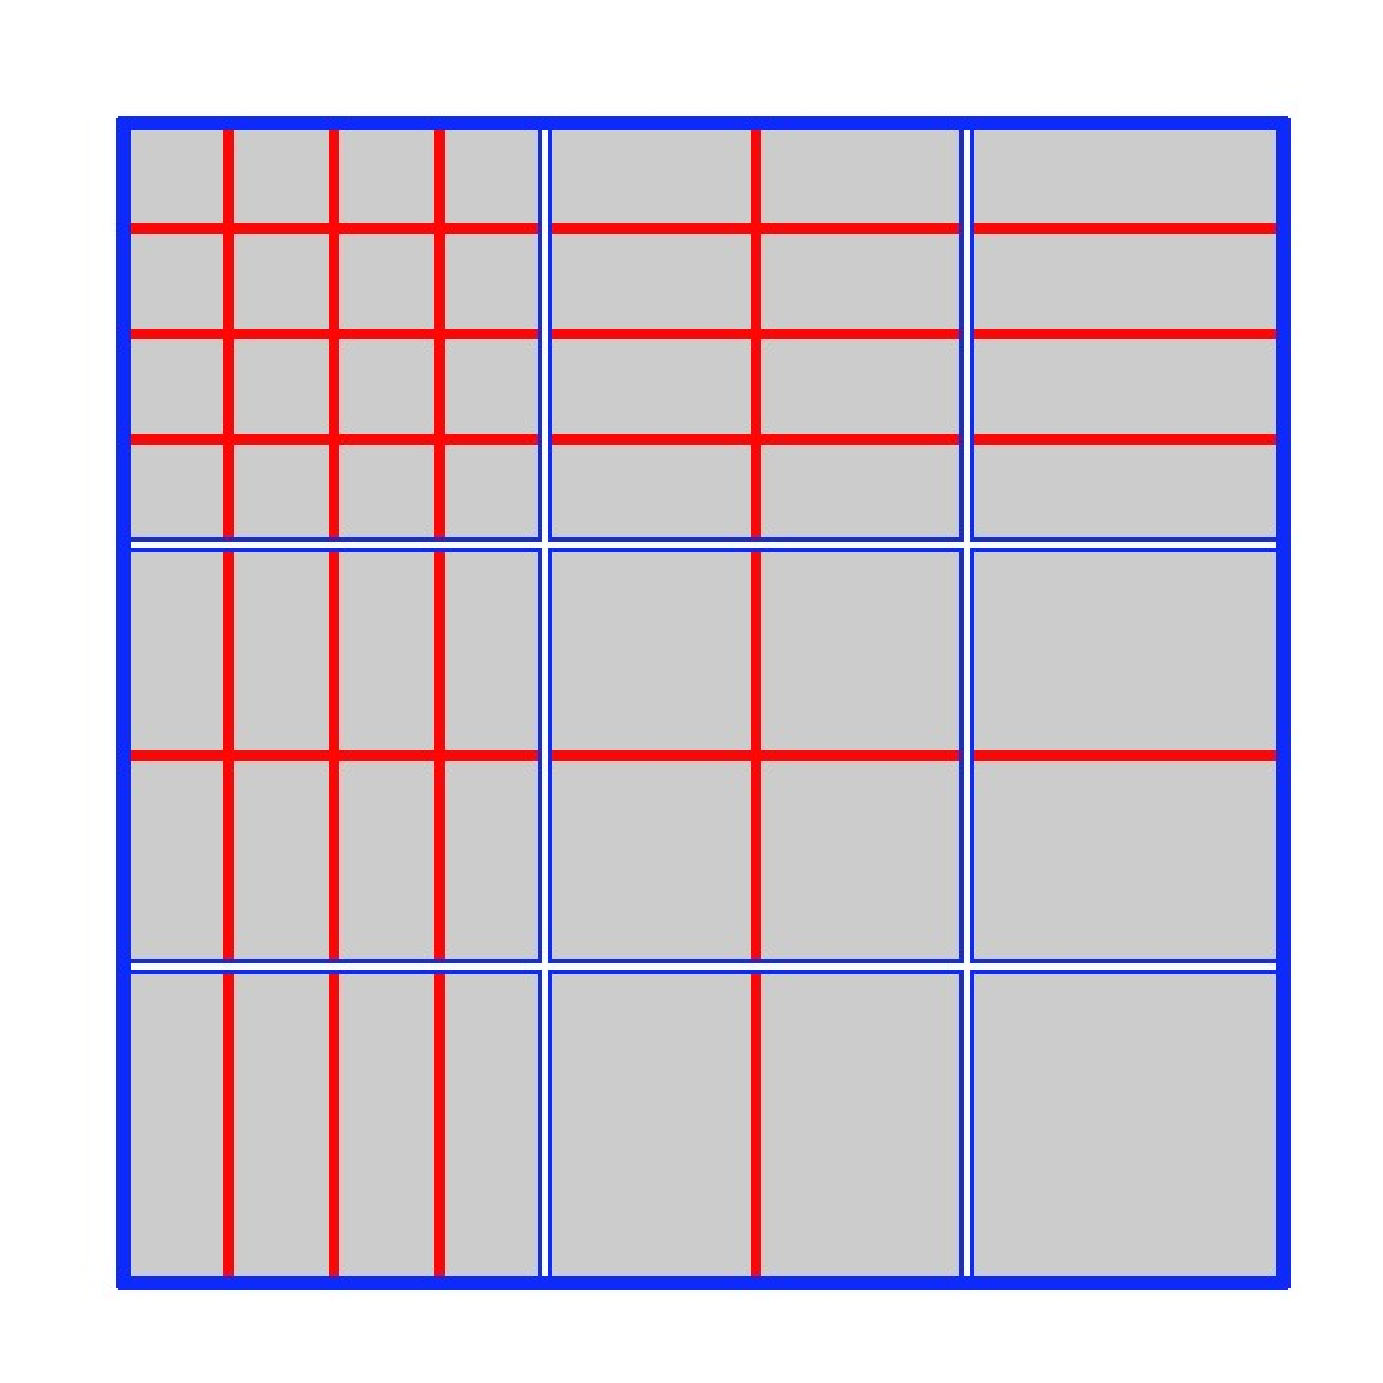
\includegraphics[scale=0.25]{block-matrix.eps}
\caption{Meta-matrix with block structure}
\label{Fock-block}
\end{center}
\end{figure}

If the programming language constructs allow, the meta-matrix can be given the usual
matrix semantics which maps individual element access to a specific
block in the submatrix.  In C++ this can be accomplished by defining
{\tt operator()(i,j)}.  The effect of this is that a complex
meta-matrix can have all: submatrix, block, and element-wise access.

The second benefit of organizing the basis set according to shells is
to allow efficient evaluation of multiple similar shell quartets on
highly parallel architectures, such as graphical processing units.
If the shells are grouped together according to coefficients and
exponents as well as the angular momentum, then evaluation of such block is guaranteed
to have the same data except for the Cartesian centers.

If the Fock matrix needs to be sorted for the computational
efficiency, the Density matrix can be permitted to reflect the desired
order.  Likewise, if other parts of the program expect Fock matrix to
be in different order, once formed, the Fock matrix can be
un-sorted.  This is especially relevant in the fock matrix is to be used
by external programs which may not necessarily sort  the basis set.


\subsection*{Collapsing Fock Algorithm Loops}
The regular Fock matrix algorithm, listing \ref{Fock:loop},
become  cumbersome if the work has to be divided between
different parallel domains and different processors/accelerators.
To make work distribution easy to implement and efficient, the four
nested loops of the Fock algorithm can be collapsed into a single
queue-like generator, listing \ref{Fock:task}.  The basic idea is to
map a single index back to four loop indices.

The advantage of using queue rather than nested loops is that queue
can be transparently and easily parallelized.
It should be noted that for the Fock algorithm, the queue tuples are
generated on the fly, rather than stored at the expense of $N^4$ tuples.

The internal counter employed in the queue can be a generic counter, for
example distributed read-modify-write counter, which allows to easily
transform the seemingly single-node queue into a distributed queue.

\begin{table}
\begin{tabular}{ p{6in} }
\hline
\begin{verbatim}
for l in N {
  for j in N {
    for k in max(l,j):N {
      for i in j,k+1 {
          ...
      }
    }
  }
}
\end{verbatim} \\
\hline

\label{Fock:loop}
\caption{Fock looping}
\end{tabular}
\end{table}



\begin{table}
\begin{tabular}{ p{6in} }
\hline
\begin{verbatim}
class Queue {
    // initial values
    counter = 0;
    last = 0;
    (i,j,k,l) = (0,0,0,0); 
    def next() {
        next = (i,j,k,l);
        end = (counter++)+1; // advance counter
        for last:end {
            if (empty()) throw exception; // signal if empty
            next = (i,j,k,l);
            i += 1; // i loop
            advance = (i >= (k+1)); // k loop
            if (advance) {
                k += 1;
                i = j;
            }
            advance = advance and (k == N); // j loop
            if (advance) {
                j += 1;
                k = max(j,l);
                i = j;
            }
            advance = advance and (j == N); // l loop
            if (advance) {
                l += 1;
                j = 0;
                k = max(j,l);
                i = j;
            }
        }
        last = end;
        return next;
    }
}
...
while (true) {
    try: (i,j,k,l) = queue.next(); // get next tuple to evaluate
    catch: break; // the end, break from the loop
    ...
}
\end{verbatim} \\
\hline

\label{Fock:task}
\caption{Fock task queue}
\end{tabular}
\end{table}


\subsection*{Exchanging bra/ket order}
Most of the integral algorithms, including Rys Quadrature, prefer the
integrals to be in such order that $A => B, C => D, A => C$.
Exchanging the order inside the integral code adds complexity and has a
performance penalty.  But for the purposes of Hartree-Fock, exchanging
the order of quartet index tuples alone and of the corresponding matrices is a
sufficient.  However, the screening must be done before changing the
order if using unmodified screening loop structure.


\subsection*{Normalization Coefficients}
Integrals beyond the $P$ shell must be normalized.  The normalization
can either be done in the integrals themselves or by absorbing the
normalization coefficients into other terms.  The advantage of
removing normalization coefficients from integrals is simpler integral
code, devoid of handling coefficients.

For the purposes of Fock algorithm, the following approach can be used
to shift normalization coefficients from integrals to Fock and Density
matrices:

\begin{eqnarray}
F_{ij} = (N_i N_j N_k N_l <ij|kl> ) D_{kl} \\
D^*_{kl} = (N_k N_l) D_{kl} \\
F^*_{ij} = <ij|kl> D^*_{kl} \\
F_{ij} = (N_i N_j) F^*_{ij}
\end{eqnarray}

Therefore, normalization can be handled by first normalizing the
Density matrix, performing regular Fock algorithm, and normalizing
the resulting Fock matrix.



\subsection*{Multithreaded Implementation}
Multithreaded Fock algorithm allows to reduce the memory overhead by
maintaining only a single copy of Fock and Density matrices per node.
The Density matrix, which is read-only, does not need to be protected
from conflicting updates.  However, the Fock matrix is subject to
conflicting simultaneous updates from multiple threads, known as race
conditions.  For example, evaluating integral tuples $(i,j,k,l)$ with
values $(1,1,4,4)$ and $(1,1,3,3)$ requires update to Fock elements
$F(k,l) = F(1,1)$ in both cases.  if the two integral tuples are to be
evaluated by two distinct threads, the access to Fock elements must be
synchronized as to avoid race conditions.

There is a number of ways this can be accomplished.  For the best
performance an approach using matrix block lock/mutex was chosen.  Since
the entire Fock matrix can be arbitrarily partitioned into blocks,
each block can be given its own mutex which is locked when a thread is
ready to update the corresponding block.  However it is wasteful to
lock the entire Fock matrix block while the integrals are being
computed and contracted.  A better the alternative is for each thread
to maintain up to six Fock buffers, $F(i, j) ... F(j,l)$, which can
then be accumulated into the main shared Fock matrix.

The algorithm outline is listed \ref{Fock:shared}

\begin{table}
\begin{tabular}{ p{6in} }
\hline
\begin{verbatim}
for (i,j,k,l) in ERI {
    // thread buffers
    Submatrix f(i,j), ..., f(j,l)
    (f(i,j), ..., f(j,l)) = Contract(Integral(i,j,k,l), D)
    // accumulates submatrix
    for f(m,n) in ((f(i,j), ..., f(j,l))) {
        F.lock(m,n)
        F(m,n) += f(m,n)
        F.unlock(m,n)
    }
}
\end{verbatim} \\
\hline
\label{Fock:shared}
\caption{Shared Fock updates}
\end{tabular}
\end{table}


\section*{C++ Implementation Details}
Since the code was written in C++ the following  libraries and
techniques were available:

\begin{itemize}
\item Boost libraries \cite{boost}
 \item {C++ meta-programming \cite{abrahams_c_2005}, including
   {\tt boost::enable\_if} \cite{boost:enable_if} and
   {\tt boost::mpl} \cite{boost:mpl}
 }
\item C99 preprocessor and Boost Preprocessor \cite{boost:pp}
\item OpenMP \cite{boost:thread}
\end{itemize}

The project relies heavily on template meta-programming
to accommodate compile time requirements of the integral and  Fock
kernels and to reduce the amount of boiler-plate code.

Various preprocessor tricks of Boost Processor are used heavily as
well.  For example, to ``transform'' a runtime value into compile time
value, the Boost Preprocessor can be used to generate the
transformation, e.g. listing \ref{braket2}.  {\tt
  BOOST\_PP\_SEQ\_FOR\_EACH\_PRODUCT} will apply a macro {\tt ERI} for
each Cartesian 4-product of shell types, essentially automatically
creating all possible handlers for quartet followed by a special case
if quartet is invalid.

\begin{table}
\begin{tabular}{ p{6in} }
\hline
\begin{verbatim}
#define TYPES (SP)(S)(P)(D)(F)//...

void runtime(Quartet quartet) {
    type a = quartet[0];
    type b = quartet[1];
    type c = quartet[2];
    type d = quartet[3];

#define ERI(r, types) \
    if (a == BOOST_PP_SEQ_ELEM(0, types) &&		\
        b == BOOST_PP_SEQ_ELEM(1, types) &&		\
        c == BOOST_PP_SEQ_ELEM(2, types) &&		\
        d == BOOST_PP_SEQ_ELEM(3, types)) {		\
        typedef shell_pair<BOOST_PP_SEQ_ELEM(0, types),      \
                           BOOST_PP_SEQ_ELEM(1, types)> bra; \
        typedef shell_pair<BOOST_PP_SEQ_ELEM(2, types),      \
                           BOOST_PP_SEQ_ELEM(3, types)> ket; \
        eri<bra,ket>(quartet);

    BOOST_PP_SEQ_FOR_EACH_PRODUCT(ERI, (TYPES)(TYPES)(TYPES)(TYPES))
    {
        throw invalid_quartet();
    }
}
\end{verbatim} \\
\hline

\label{braket2}
\caption{Using preprocessor}
\end{tabular}
\end{table}


The multithreading was done using OpenMP.  While Boost Thread library
is much more powerful and versatile than Openmp, only a subset of
multithreading constructs were needed to make code multithreaded,
primarily loop counter synchronization and mutex constructs.

Besides the above-mentioned libraries, other miscellaneous components
from Boost and Standard Template Library were used throughout the project.  



\section*{GPU Implementation}

Oover the years there have been various implementations of integral
quotations using GPU's, for example McMurchie-Davidson
\cite{ufimtsev2008quantum}, \cite{ufimtsev2009quantum}, Rys Quadrature
\cite{yasuda2008two}, \cite{wilkinson_acceleration_2011}.  The above
implementations primarily targeted single precision computations with
$Ss,p$ functions only, using either CUDA C or accelerator statements.
The Current generation of the gpu hardware has much smaller difference
in single-vs-double precision, making the case for single precision
less obvious.  

Our approach was to utilized double precision
exclusively to reproduce the CPU results and to go well beyond the $s,
p$ functions. The GPU implementation was done using NVIDIA CUDA technology.
To best understand the subsequent details, one needs to be
familiar with the CUDA terminology, cf. CUDA Programming Guide.

In developing the GPU implementation of the Hartree-Fock method, the
 following factors are considered:
\begin{itemize}
\item High angular momentum and low angular momentum/highly
  contracted integrals are different in nature to warrant different
  implementation approaches.
\item The integral kernels must evaluate many batches of integrals
  in one launch.  By sorting the basis, a large number
  of quartets, differing only in centers, but not in shell primitives,
  can be generated..
\item The integrals must be contracted with density $D$ as soon as
  possible to reduce memory overhead from $n^4$ to $n^2$.  Therefore
  the entire integral quartet is never written into the device memory.
\item Contracting integrals with the density directly results in
  race conditions which must be accounted for.
\item Integral batches which can not be evaluated on the device, must
  be done on the host.
\end{itemize}

The current Fermi hardware has 32768 registers and 48KB of shared
memory.  The number of concurrent thread blocks is 8.  A typical
integral kernel will use around 60 registers per thread and 6KB of
shared memory. Therefore, up to 8 thread blocks can be executed
simultaneously, 64 threads each.  The 64 threads are executed in
warps, 32 threads per warp.  The threads in warp are implicitly
synchronized but their execution is not implicitly synchronized with
the other warp.  In essence, warp can be thought of as an
independently executing unit. This fact can be used to partition
work along the warp boundaries.

The development of integral kernels follows the CPU version closely:
the implementation is split into a general and low angular momentum
kernels.  The latter is parallelized over the contraction loop, the
former over the integral elements primarily.

In both cases, the efficient implementation demands that the type of
integral be known at compile time.  This is handled by implementing
integrals using C++ templates, with the braket type being a compile
time parameter and the shell exponents and coefficients a runtime parameter.

The shells, centers, and quartet lists are stored in the device
memory.  Regardless of implementation, each kernel loads all three and
forms the corresponding bra/ket primitives in shared memory.

\subsection*{General Integral Kernel}
The general integral kernel is applicable to (nearly) all combinations
of contraction order and the braket types.  While the general kernel
may not perform equally well for some combinations, those combinations
can be handled by specialized kernels and chosen instead at the
runtime.

There are multiple ways one can approach the problem of
implementing a general Rys Quadrature on GPU with its limited
resources.  Our approach is along the following general lines:

All roots and weights are computed first and stored in the shared
memory.

Each thread is assigned a 3-D index corresponding to recurrence and
transfer computation it will perform.  The x-index corresponds to
either bra or ket index, y and z indices corresponds to Cartesian
index and root index respectively.  In general, $(L_{ab}+1)*3*N$
threads are needed, where $L_{ab}$ is the bra angular momentum and $N$
is the number of roots.  In certain cases not all recurrence/transfer
computations are needed and then that number may be $(L_{ab})*3*N$.

The computations are independent of one another in y and z indices, but are
dependent on the previous results of a thread with another x-index
(and same y,z index).  Consider the graphical depiction of a transfer
relation to form $(fd|$ intermediate, Fig \ref{transfer}.  The intermediate
$(4,2)$ computed by thread $4$ depends on value of $(5,1)$ computed by
thread $5$.  To ensure correctness, the work of both threads must be
synchronized.  If the threads are aligned to $2^n$ boundaries,
synchronization is implicit.  What that means is that if the overall number
of threads needed is $(L_{ab}+1)*3*N$, padding $(L_{ab}+1)$ to a power
of 2 will ensure that all threads with the same $y,z$ index are in the
same warp at the (miniscule) expense of some idle threads.

\begin{figure}[here]
\begin{center}
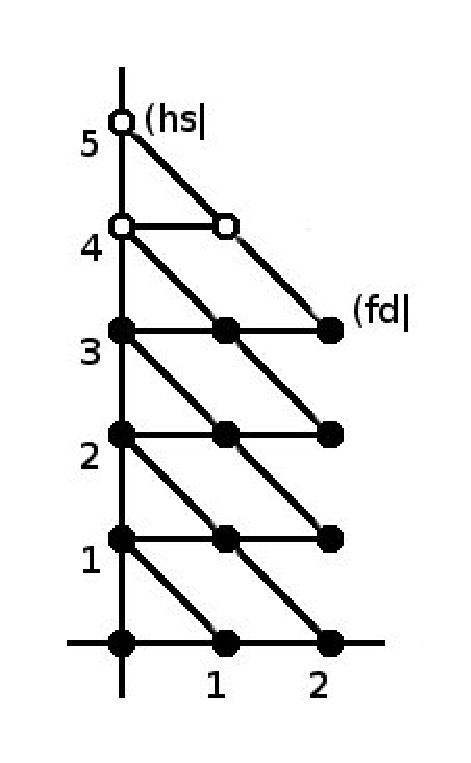
\includegraphics[scale=0.5]{transfer.eps}
\caption{Transfer diagram to form $(fd|$ bra}
\label{transfer}
\end{center}
\end{figure}

There are three ways the mappings can be aligned to warp:
\begin{itemize} 
\item The entire reccurence/transfer computation (if small enough) is
  mapped to a warp (or half-warp or quarter-warp, etc).  This holds if
  $(L_{ab}+1)*3*N <= warp$.
\item The xy dimension is aligned to a $2^n$ boundary. For example, if
$L_{ab} = 5$, the xy-boundary is 16 threads.
\item The x dimension is aligned to a $2^n$ boundary.  For example, if
$L_{ab} = 7$, the x-boundary is 8 threads.
\end{itemize}

the first option is preferred. If the first condition fails, the choice
between the latter two depends on which minimizes the overall thread count.
For example, if $L_{ab} = 5$, the second alignment needs 16 threads,
versus 24 threads.  If $L_{ab} = 7$, the second alignment needs 32
threads, while the third needs 24.

Once the intermediates are ready in the shared memory, each thread
computes a subset of integrals.  The mapping between thread/integral
index and the corresponding 2D integrals index is stored in the main
memory and looked up for each element.  The index is stored in a
four-element vector, with the fourth index containing coefficient
index for hybrid SP functions.
 
Once all the integrals are formed, they are transferred to shared
memory, previously used to store roots and intermediates.
The exact number of integrals each thread computes depends up on the
size of integral quartets and the number of threads launched.  The
number of threads depends mostly on the dimensions of
recurrence/transfer computations and amount of shared memory used by
the kernel.  To accommodate those two requirements, a number of
kernels is available with either 2, 3, 4, or 8 multiples of warp
and the corresponding number of integrals per thread.  During
runtime the kernel which maximizes the device occupancy is chosen.

In the case if entire reccurence/transfer computation can be mapped to
a single warp, the integrals can be partitioned to warps rather than
to an entire thread block, with each warp assigned to evaluate a
unique contraction.

As implemented, the above approach is able to handle any quartet with
the total angular momentum of 9 or less, for example $fd|dd$,
including shells with hybrid SP coefficients.  The limit of 9 is due
to the limit of the Rys roots program.

\subsection*{Low Angular Momentum Integrals}

The most natural way to evaluate low angular momentum integrals is to
assign individual quartets to a thread block, and a single contraction
to a thread, with each thread evaluating all integral elements
corresponding to that contraction.  However, this scheme becomes
inefficient if the number of contractions is the smaller than the
number of threads in block.  This problem can be partially solved by
assigning individual roots, rather than contractions, to a thread.
For example, for $(ps|ps)$ quartet this effectively doubles the number
of tasks to distribute as per each contraction there are two roots
generated.

The low angular momentum kernels reuse the CPU kernel verbatim, with
each device thread evaluating an individual root and all of the
corresponding integrals, subsequently reduced into shared memory.

Once implemented, the above approach was still insufficient to saturate
the threads.  With a slight modification, the
above implementation was modified to handle an individual quartet per
warp, in essence assigning two quartets per thread block.  As an
additional benefit, shell primitive loads decreased by half.

\subsection*{GPU Hartree-Fock Implementation}
It is not possible to implement a parallel version of Fock contraction
within a thread block where all six Fock contributions can be
evaluated in the single inner loop.  The approach taken was to split the
six updates onto separate loops, such that each Fock element can be 
 computed independently. \\
The implementation is as follows:

\begin{itemize}
\item One of the six integral/density loops is mapped to warp.
  Hence one thread block can contract and store one or more Fock
  tiles corresponding to the integral batch concurrently.
\item The individual Fock elements are mapped uniquely to a thread in a warp.
\item The warp loads density tile into shared memory.
\item The density tile is contracted with integral batch and the 
  Fock element is stored in a register.
\item The  Fock matrix is locked with exclusive r/w lock and
  a Fock element is added to device memory
\item The mutex is unlocked and warp proceeds to contract the next tile.
\item Both, the density and Fock tiles are stored in a block manner, such
  that all elements of a tile are continous in memory.
\end{itemize}


\begin{table}
\begin{tabular}{ p{6in} }
\hline
\begin{verbatim}
lock(i,j) {
  while (atomicCAS(mutex(i,j),1)) {}
}
unlock(i,j) {
  mutex(i,j) = 0;
}

fock (i, j, k, l) {
  shared G; // integrals
  shared d(k,l); // density tile
  d(k,l) = D(k,l); // load density tile
  f = contract(g,d); // contract
  lock(i,j); // obtain lock
  F(i,j) += f; // add to main memory
  unlock(i,j); // release lock
}

if (do_ij) fock(i, j, k, l);
if (do_kl) fock(k, l, i, j);
if (do_ik) fock(i, k, k, l);
if (do_il) fock(i, l, k, l);
if (do_jk) fock(j, k, i, l);
if (do_jl) fock(j, l, i, k);

\end{verbatim} \\
\hline

\label{gpu-fock}
\caption{GPU HF kernel}
\end{tabular}
\end{table}


Only one contraction out of six has a simple indexing,
the other five contractions traverse the integrals
with non-contiguous stride, which must be accounted for.

The current CUDA implementation does not provide built-in device
memory mutex, however mutex can be implemented with atomic compare and
swap operation, {\tt atomicCAS}.  The mutex implementation above will
spin until a zero is read.  Rather than locking the entire Fock
matrix, only the individual tiles are locked at a time. \\

To achieve performance in the presence of mutex, the quartets must be
traversed so that the indices are not too similar, as it would lead to
mutex contention.  E.g. processing quartets $(0,0,0,0), (1,0,0,0),
...$ would result in high number of collisions as integrals quartets
are prescreened sequentially.  This problem can be solved by
traversing the quartet list in non-one strides, for example in strides
of 32 in round-robin manner, provided the quartet lists are on the
order of thousands of entries.  Since the basis set is sorted to begin
with, the generated integral lists are typically well into thousands.

\subsection*{Host/GPU Integration}
The gpu device is driven by a separate host thread.  Upon the start,
density matrix is copied into the device memory and Fock matrix is
initialized to zeros.  GPU thread requests a task from a task queue.
If the quartet task can be evaluated by a device kernel, the quartets
are prescreened on the host, asynchronously copied to device and the
kernel is launched, asynchronously as well.  This leaves the host
thread to either prescreen the next batch or to evaluate quartets
which can not be handled on the device.  This allows for overlap of
cpu/gpu execution.  As will be shown in the performance section, the
number of unhandled quartets is small, even with a high angular
momentum basis.  Once the tasks are exhausted, the device Fock matrix
is merged into the host.


\section*{Performance}
The newly implemented Fock algorithm was compared against the
standard GAMESS \cite{gamess} code, using Rys Quadrature only
and the default GAMESS option which picks an optimal integral package,
eg \cite{ishimura}. \\
The GAMESS code was compiled with the following command:\\
{\tt gfortran -O3 -msse3}\\
The new implementation was compiled with:\\
{\tt g++ -O3 -msse3}

The gcc version was 4.4.3 for both, gfortran and g++.
the benchmarks were run on two Intel Xeon E5405, 2.00GHz, CPUs.

The results are listed in Table \ref{results1}. All the timings are in seconds.
Except for the results of the last column, GAMESS was set to utilize a single
core. The last column lists the results of running eight threads
to utilize all cores.
The following has to be kept in mind interpreting the results:

\begin{itemize}
  \item The rotated axis algorithm and its variations are
    algorithmically much less complex than Rys Quadrature for
    contracted shells, like those typically found in low angular
    momentum basis sets.
\item The rotated axis code \cite{ishimura} in GAMESS has been
  re-implemented only three years ago and should hypothetically take
  advantage of modern processors.
\item Rys Quadrature is advantageous for small contraction high
  angular momentum basis sets.  The implementation of Rys Quadrature
  found in GAMESS is the original implementation from the HONDO
  \cite{hondo} package and does not take into account modern processor
  architecture.
\item For large basis sets with $f$ functions the relative number of
  shell quartets handled by Rys Quadrature is significantly higher.
\end{itemize}

The test computations were performed on Cocaine, Taxol, and
Valinomycin molecules using the basis sets that incorporate a
different number of $s$, $p$, $sp$, $d$, and $f$ shells.  Notice that
Cocaine is smaller of the three and Valinomycin is the larger.  The
improvement over the original Rys Quadrature is on the order of
30-40\%.  When compared to default integral option in GAMESS, which
does not pick Rys Quadrature if no $f$ functions are present, the
performance is either higher, lower, or the same, depending on the
number of $d$ functions, the size of the basis and correspondingly the
memory requirement of density and Fock matrices.

The rewritten Rysq Quadrature is still much slower than the
rotated-shell axis code when only $s, p$ functions are involved, the
difference most pronounced when the total basis set is small.  The
difference diminishes with increasing Fock and density matrix sizes as
the memory locality becomes more important.  For example, with small
Cocaine 6-31G compuation the rotated shell axis code is 75\%
faster, but only 30\% faster with much larger Valinomycin 6-31G
compuation.

With the $d$ functions present the C++ Rysq Quadrature code performs
 better than the current packages as the basis size
increases.  With Taxol and Valinomycin it outperforms the current
GAMESS codes by few percent.

The new code clearly becomes faster if the $f$ functions are present.
In the best case scenario, it is 31\% faster than GAMESS integral
packages, due to both, better memory locality and the higher fraction
of quartets with higher angular momentum.

From these results the following can be gathered:
\begin{itemize}
  \item A well-designed code {\it can} be competetive with
    algorithms which have lower computational complexity.
  \item A well-designed C++ program can be as fast or faster than a
    Fortran program.
  \item The new Hartree-Fock implementation is scalable and efficient,
    both memory-wise and computer-time wise, improving the overall
    performance by as much as 30\%.
\end{itemize}

\begin{table}
  \label{results1}
  \caption {C++ CPU performance}
  \begin{center}
    \begin{tabular}{| l | c | c | c | c |}
      \hline
 Input                    & GAMESS & GAMESS/Rys & C++ & Improvement (\%) \\
 \hline
 Cocaine 6-31G            & 21.3   & 52.4   & 37.2   & -74.6/29.0 \% \\ 
 Cocaine 6-31G(d)         & 65.0   & 112.9  & 75.2   & -15.7/33.4 \% \\ 
 Cocaine 6-31G++(d,p)     & 402.7  & 592.0  & 405.1  & -0.60/31.6 \% \\ 
 Cocaine 6-311G++(2df,2p) & 3424.4 & 3686.4 & 2356.3 &  31.2/36.1 \% \\ 
 \hline
 Taxol 6-31G              & 310.2  & 691.6  & 474.1  &  -52.8/31.4 \% \\
 Taxol 6-31G(d)           & 1104.2 & 1729.2 & 1040.0 &    5.8/39.8 \% \\
 Taxol 6-31G++(d,p)       & 11225.9 & 15380.5 & 10288.0 & 8.4/33.1  \% \\
 \hline
 Valinomycin 6-31G        & 853.6  & 1700.7 & 1104.4 & -29.3/35.3 \% \\ 
 Valinomycin 6-31G(d)     & 2285.0 & 3445.7 & 2104.8 &   7.9/38.9 \% \\
 \hline
    \end{tabular}
  \end{center}
\end{table}

The comparison between the C++ CPU and GPU codes is in tables
\ref{results2}, \ref{results3}, \ref{results4}, broken down by the
relative time a particular shell quartet takes.  For example,
$(ps|ss)$ quartets are of size 3 and $(dd|dd)$ quartets are of size
1296. The benchmark molecule is Taxol and the three basis sets are
cc-PVDz , cc-PVTz, and 6-31G(d) \cite{davidson_basis_1986}.
  The correlation consistent basis have contraction order
as high as 4096 while the Pople basis rely heavily on hybrid $sp$
shells.  It should be noted righ away that a large fraction of
integral time is spent computing the multitude of integrals with $p$
shells.  In fact, for the CC-pvDZ basis, 60\% of total time is spent
evaluating the smallest four integrals.

The speed-up varies, from 17.5x to 12x for the cc-PVTz basis.
The specialized low-angular momentum quartet kernels perform fairly
well, with the lowest speed-up for the last specialized kernel with
two $sp$ shells, size 16.  The speed-up consequently drops as the
general kernel.  The performance picks up as the quartet gets bigger.
The number of slower kernels in 16 to 100 range is rather high and it
yends to lower the overall speed-up.   

\begin{table}
  \label{results2}
  \caption {Taxol/CC-PVDZ GPU performance}
  \begin{center}
    \begin{tabular}{| l | c | c | c |}
      \hline
      quartet size & CPU \% by time  &  speed-up (x)\\
      \hline
      1 & 14.2 & 35.2 \\
      3 & 22.8 & 23.0 \\
      6 & 6.6 & 18.5 \\
      9 & 19.3 & 17.4 \\
      18 & 9.6 & 14.5 \\
      27 & 7.0 & 9.6 \\
      36 & 1.6 & 11.4 \\
      54 & 8.7 & 12.6 \\
      81 & 1.9 & 12.8 \\
      108 & 3.3 & 17.2 \\
      162 & 2.5 & 16.0 \\
      216 & 0.4 & 14.3 \\
      324 & 1.6 & 16.7 \\
      648 & 0.4 & 17.9 \\
      1296 & 0.1 & 15.0 \\
      \hline
      overall & 5068.66 s &  17.5 \\
      \hline
    \end{tabular}
  \end{center}
\end{table}


\begin{table}
  \label{results3}
  \caption {Taxol/CC-PVTZ GPU performance}
  \begin{center}
    \begin{tabular}{| l | c | c | c |}
      \hline
      quartet size & CPU \% by time  &  speed-up (x) \\
      \hline
      1 & 4.3 & 25.9 \\
      3 & 8.5 & 17.5 \\
      6 & 4.6 & 15.1 \\
      9 & 8.4 & 13.8 \\
      10 & 1.7 & 14.6 \\
      18 & 8.0 & 11.6 \\
      27 & 3.7 & 8.2 \\
      30 & 3.7 & 9.3 \\
      36 & 2.5 & 10.4 \\
      54 & 8.3 & 11.4 \\
      60 & 2.5 & 13.3 \\
      81 & 1.1 & 11.4 \\
      90 & 4.1 & 15.1 \\
      100 & 0.8 & 15.5 \\
      108 & 5.8 & 15.9 \\
      162 & 2.9 & 15.0 \\
      180 & 5.2 & 14.0 \\
      216 & 1.2 & 14.1 \\
      270 & 1.7 & 17.3 \\
      300 & 1.4 & 15.8 \\
      324 & 3.5 & 17.3 \\
      360 & 1.7 & 15.4 \\
      540 & 3.6 & 18.9 \\
      600 & 1.1 & 15.7 \\
      648 & 1.6 & 17.9 \\
      900 & 1.1 & 18.7 \\
      1000 & 0.2 & 15.0 \\
      1080 & 2.9 & 15.3 \\
      1296 & 0.4 & 15.8 \\
      1800 & 1.6 & 19.4 \\
      2160 & 0.7 & 20.1 \\
      3000 & 0.3 & n/a \\
      3600 & 0.7 & n/a \\
      6000 & 0.3 & n/a \\
      10000 & 0.0 & n/a \\
      \hline
      overall & 35110.4 s &  12.0 \\
      \hline
    \end{tabular}
  \end{center}
\end{table}


\begin{table}
  \label{results4}
  \caption {Taxol/6-31G(d) GPU performance}
  \begin{center}
    \begin{tabular}{| l | c | c | c |}
      \hline
      quartet size & CPU \% by time  &  speed-up (x) \\
      \hline
      1 & 1.7 & 28.5 \\
      4 & 6.5 & 20.9 \\
      6 & 1.9 & 18.8 \\
      16 & 12.3 & 13.1 \\
      24 & 6.6 & 10.6 \\
      36 & 1.1 & 11.7 \\
      64 & 13.9 & 13.7 \\
      96 & 16.8 & 15.8 \\
      144 & 5.9 & 19.5 \\
      216 & 0.6 & 15.4 \\
      256 & 12.4 & 23.5 \\
      384 & 11.5 & 20.9 \\
      576 & 7.0 & 20.2 \\
      864 & 1.7 & 21.3 \\
      1296 & 0.2 & 16.6 \\
      \hline
      overall & 1031.94 s &  16.6 \\
      \hline
    \end{tabular}
  \end{center}
\end{table}


\section*{Conclusions}
The newly implemented Rys Quadrature and Fock Matrix  algorithms,
implemented as a stand-alone C++ library, with C and Fortran bindings,
shows on the order of  40\% improvement over the traditional Fortran
Rys Quadrature and the performance similar to that of less
computationally intensive algorithms.  The library is fully
multithreaded and has favorable scaling across eight cores.

The GPU version, adopted from the CPU version, shows speed-up as high
as 17.5x.  The Rys Quadrature however does not scale well in the
mid-size shell quartets.  Port of a Rotated-Shell axis code is likely
to increase the overall performance to 20X or higher.

\bibliographystyle{unsrt}% (uses file ``plain.bst'')
\bibliography{references}
\documentclass{beamer}
\usepackage[latin1]{inputenc}
\usetheme{Warsaw}
\title[ Software Design In Computational Sciences]{Software Design In Chemistry}
\author{ Andrey Asadchev}
\institute{Iowa State University}
\begin{document}

\begin{frame}
\titlepage
\end{frame}


\begin{frame}{Outline}
\begin{itemize}
\item Programming Languages
\item Object Oriented Programming
\item C++ and Python
\item Symbolic Computation
\item Current Computer Architectures
\item Computational Chemistry
\item Integral Evaluation
\item Fock Matrix
\item GPU Implementation
\item Performance
\item Conclusions
\end{itemize}
\end{frame}

\begin{frame}{Programming languages}
\begin{itemize}
\item Communicate To Computer And To Humans
\item Binary Machine Language - instructions as sequence of zero and one
\item Assembly - mnemonic shortcuts to machine language
\item Fortran - early imperative programming language.\\
  Numerical and matrix computations.
\item LISP - functional programming language.\\
   Stands for List Processor.\\
   Functions (as in mathematics) are first-class citizens.\\
   To Iterate Is Human, To Recurse Is Divine.\\
   Lambda functions and predicates: $G = map(lambda\, x,y: x*y, F,reversed(G))$\\
   Artificial Intelligence\\
\item C - Portable Assembly Language.\\
  developed together with UNIX operating system.\\
  System Programming Language.\\
  Access to the raw memory.
\end{itemize}
\end{frame}



\begin{frame}{ Object-Oriented Programming}
\begin{itemize}
\item Abstract implementation problem 
\item Keep Data and Methods together
\item Hide Data, Puts Constraints on Data
\item Polymorphism 
\item Inheritance
\item Matrix\\
Represented As Some Object M\\
M.transpose()\\
const M.m\\
Orthogonal Matrix Is a Matrix\\
Orthogonal Matrix Has Transpose\\
Orthogonal Matrix  has inverse\\
\end{itemize}
\end{frame}


\begin{frame}{  C++}
\begin{itemize}
\item Superset of C
\item Object Oriented
\item Functional
\item Widely Used, Many Compilers
\item Efficient, games programming and digital signal processing
\item Overload operators, + , *,...
\item Program formulas almost like on the paper\\
$Vector\, r = v-w $\\
\item Template meta-programming\\
 Generic Programs\\
 Automatically Generated Programs\\
 Specialized Programs\\
 Boost\\
Domain Specific Language And Template Expressions\\
Readability: $Quartet \langle Shell \rangle$
\end{itemize}
\end{frame}

\begin{frame}{  Python}
\begin{itemize}
\item Interactive,compiled 
\item Imperative
\item Object Oriented
\item Functional
\item Easy interfacing with other languages
\item Pythonic\\
 L = sorted([(x,y) for x in X for y in Y if x is y])
\item Widely Used in Science and Mathematics\\
pyQuante
\item  Template-preprocessor engines (PHP)\\
  Cheetah\\
Preprocessor directives directly embedded in program\\
\end{itemize}
\end{frame}

\begin{frame}{ Symbolic computations}
\begin{itemize}
\item Computed Expressions Without Explicitly Knowing Number
\item Computer Algebra Systems
\item Mathematica.\\
  Polynomial Manipulation\\
Matrix Manipulation\\
Recursion\\
Allows to Define Your Own Algebra\\
\item  Sage.\\
    Python Computer Algebra System\\
    Interface to almost any other computer algebra system
\item Sympy - symbolic python library.\\
\item  Put Equations As They Are.\\
Let Computer Algebra System Simplify Them\\
Use Program Generator to produce code as you  wanted\\
Optimize equations which otherwise would be prohibitive to
\end{itemize}
\end{frame}

\begin{frame}{ Computer Architecture}
\begin{itemize}
\item Pipeline
\item Single Instruction Multiple Data
\item Memory Locality
\item Many cores
\item Complex Scheduling
\item Very Hard to Beat a Compiler for Low-Level Optimization\\
however programs have to be written in such way as to be amenable to optimization\\
Conditional statements, unpredictable memory access prohibit optimization.
\item Processors Are Powerful and Cheap\\
     Optimized for Games and Signal Processing, 4x4 matrix\\
     Underutilized often, 15 percent efficiency is common
\item  Efficient Implementations demand unrolling kernels
\end{itemize}
\end{frame}

\begin{frame}{ Computer Architecture}
\begin{itemize}
\item 
\item   Graphical Units\\
 A Lot Of Performance And Even More Hype\\
 Memory Bound Often\\
 Single Instruction Multiple Thread\\
 Imagine mapping each loop iteration to threads\\
 for i  = threadID,N,numThreads:  X(i) = aY(i)
\end{itemize}
\end{frame}

\begin{frame}{  Computational Chemistry}
\begin{itemize}
\item Electron Integrals $(ab|cd)$\\
  Domain Specific\\
  Define rest of computations
\item Lots of Computations, Lots of Memory
\item Data Screening, Symmetry
\item  Linear Algebra, BLAS
\item Legacy Code
\item MPQC, libint
\end{itemize}
\end{frame}

\begin{frame}{   Integral  evaluation}
\begin{itemize}
\item $(ab|cd) = \sum C_i \sum C_j \sum C_k \sum C_l [ij|kl] $
\item $(ab|cd) = (ba|cd) = (cd|ab)...$
\item many different combinations and permutations
\item SP functions
\item high angular momentum versus high confection order\\
$(fsp | fsp)$
\item gaussian basis, $e ^{-r^2}$ separable in Cartesian coordinates
\item  Most Integral schemes use recursive nature of gaussian integration/differentiation
\item Numerical error - loss of significant figures, etc.\\
Recursion implies using a slightly incorrect value to compute next\\
Especially severe when two values are close in magnitude but different in sign (difference)
\end{itemize}
\end{frame}

\begin{frame}{   Integral  evaluation}
\begin{itemize}
\item 
\item OS integral scheme, auxiliary integrals. \\
Very general - applicable to almost any operator\\
R12 linear integrals\\
Memory Hungry
\item Rys quadrature\\
  Gaussian quadrature using Rys orthogonal polynomials\\
  $I = \sum_a Ix(a)Iy(a)Iz(a)$\\
  Compute Roots\\
  Compute two-dimensional x, y, z intermediate integrals\\
  Assemble final integral
\item Horizontal recurrence\\
$(pp | = q*(ps |  + (ds |$\\
Simplifies Contracted Integrals\\
High Numerical Error
\end{itemize}
\end{frame}

\begin{frame}{  Integral Implementation}
\begin{itemize}
\item C++ object-oriented library
\item Fortran And Gamess bindings
\item  Simple Interface:\\
Create quadrature object for given shell quartet\\
Call Object operator for a given center quartet
call object operator for a list of Center quartets

\item Two Internal Implementations:\\
  Fully Unrolled And Simplified kernels for smaller  integral, 
  which is likely to be contracted\\
  Partially Unrolled (bra only) general quadrature\\
\item Internals make heavy use of  C++ templates and automatically generated code
\item Human Serviceable Code is small - around 2000 lines of code
\item Final Library Size his small - around 5 megabytes fully optimized
\item the code is kept small due to objects and genetic templates
\end{itemize}
\end{frame}

\begin{frame}{  Fock Matrix}
\begin{itemize}
\item $F = (ab |cd)D $
\item Part of the Library
\item Requires Matrix to be in block form through an adapter
\item Simple Interface:\\
Create fock object for given shell quartet\\
Call Object operator for a given center quartet\\
Call Object operator for a list of Center quartets
\item Two Internal Implementations - parallel to those of integral program
\item Basis Set organization and higher-level logic is handled by another library
\end{itemize}
\end{frame}

\begin{frame}{  GPU implementation}
\begin{itemize}
\item Implementations are driven by integral size and contraction order
\item Large integrals are parallel over individual elements\\
every thread gets a unique internal element to compute
\item highly contracted small integrals are parallel over contractions\\
every thread gets the unique contraction to compute\\
contractions are  reduced in the end
\item Basis  must be ordered to guarantee execution of the kernel on multiple centers
\item Thanks to objects and genetic templates, the entire kernel code is about 300 lines
\end{itemize}
\end{frame}

\begin{frame}{   Performance}
\begin{itemize}
\item GPU implementation not yet complete
\item CPU implementation:\\
  benchmark several cases from hundred to a thousand basis functions\\
  largest test is loperamide 6-31G(pdf)
  numerical agreement to 8 decimal places\\
  30-40\% improvement in speed\\
  Fine grain contraction screening was not enabled\\
  Intel compiler generates vector instructions\\
  still working on full optimization
\item GPU implementation not yet complete\\
  basic integrals, up to the 1500 quartet size are working\\
  50\% improvement over CPU\\
  numbers essentially agree
\end{itemize}
\end{frame}


\begin{frame}{Aknowledge}
\begin{itemize}
\item Funding From Dr. Gordon
\item  Help From Jacob and Allada
\end{itemize}
\end{frame}

\end{document}

  
\end{document}



% LocalWords:  Fock un def Multithreaded mutex ERI Submatrix bst
